%% SECTION HEADER /////////////////////////////////////////////////////////////////////////////////////
\section{Experimental setup for the \acs{hsc} model validation}
\label{sec:setup}
%% SECTION CONTENT ////////////////////////////////////////////////////////////////////////////////////
\begin{figure}[!htb]
	\begin{center}
		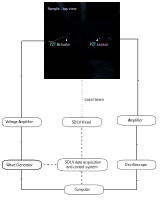
\includegraphics[width=0.95\textwidth]{Chapter_6/setup}
	\end{center}
	\caption{Experimental setup for (1) the \acf{sldv} measurement - dashed line and (2) the \acf{pzt} wave acquisition - solid line.}
	\label{fig:setup}
\end{figure}
The presented model of the \ac{hsc} was validated with results from two experimental studies.
The first one was performed for determination of the full wavefield of the propagating waves by the \ac{sldv} (Polytec PSV–400).
The second study was performed for wave acquisition by the \ac{pzt} sensor.
A schematic of the experimental setup is shown in Fig.~\ref{fig:setup}.

The \ac{sldv} is a modern method for non-contact measurement of the vibration velocity of structure surface particles.
The principle of vibrometer operation is based on the Doppler effect, recording the change of frequency of the light beam reflected from the vibrating surface.
In laser vibrometry, the measurement of frequency change is realised by interferometer and analysis of both reference and measurement light beam.
The measuring system is additionally equipped with mirrors allowing to change the angle of the measuring beam, so it is possible to take measurements at a grid of points on a surface of inspected structural element automatically.
The \ac{sldv} setup is presented in Fig.~\ref{fig:sldv}.
\begin{figure}[!htb]
	\begin{center}
		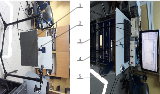
\includegraphics[width=0.95\textwidth]{Chapter_6/sldv}
	\end{center}
	\caption{The \acf{sldv} setup: 1 - the laser sensor head, 2 - the \acf{hsc} specimen, 3 - the arbitrary waveform generator, 4 - the amplifier, 5 - data management system}
	\label{fig:sldv}
\end{figure}

The \ac{pzt} elastic wave generation and acquisition system is used to measure the voltage changes of transducers due to their mechanical deformation.
It is a point measurement at the point of sensor placement.
A data management unit is responsible for executing prepared tasks and collecting data recorded during measurements.
An arbitrary waveform generator is the source of the low voltage signal, which feeds the Lamb wave detection system and high voltage amplifier.
The amplified signal is intended for the actuator to excite a wave in the sample.
The Lamb wave charge amplifier collects the registered signal by the sensor. 
Then it is supplied to an oscilloscope via a splitter.
The setup used for measurements is shown in Fig.~\ref{fig:pzt_setup}.
\begin{figure}[!htb]
	\begin{center}
		\includegraphics[width=0.95\textwidth]{Chapter_6/pzt_setup}
	\end{center}
	\caption{The \acf{pzt} setup, (\textbf{a}) the elastic wave generation and acquisition instruments:  DMU - the data management unit, G1,G2 - the arbitrary wave generator, O - the oscilloscope, HVA - the high voltage amplifier, LWDS - the Lamb Wave Detection Systems, (\textbf{b}) the specimen with the pair of \ac{pzt}.}
	\label{fig:pzt_setup}
\end{figure}

Both methods have some advantages and disadvantages, which are given in the Table~\ref{tab:method_comp}.
The best advantage is of the \ac{sldv} technique is a non-contact surface measurements.
If three heads of the laser sensor are available then three-axes of velocity measurements are possible. However, due to the large size of the setup, and the high signa-to-noise ratio it is used in laboratory conditions.
On the hand the \ac{pzt} setup is a rather low cost instruments for spot recording of the wave propagation.
The measurements are characterized by high repeatability and can be performed on the construction in operation.

\begin{table}[!htb]
	\small
	\tabcolsep=0.2cm
	%\centering
	\caption{\label{tab:method_comp}Comparison of methods for elastic wave propagation measurements.}
	\begin{tabular}{p{0.1\textwidth}>{\raggedright}p{0.4\textwidth}>{\raggedright \arraybackslash}p{0.4\textwidth}}
		\toprule
		\textbf{Method} &\textbf{Advantages} & \textbf{Disadvantages}\\
		\midrule
		\multirow{5}{*}{\ac{sldv}}   & \tabitem automatic full-field scanning & \tabitem high-cost equipment\\ 
		& \tabitem non-contact measurement & \tabitem long measurement time\\
		& \tabitem \ac{3d} velocity vector (optional)& \tabitem special surface treatment is needed to avoid scattering of the laser beam, e.g. by application of retro-reflective tape\\
		& & \tabitem high signal-to-noise ratio\\
		& & \tabitem relatively large space need for measurements \\
		& & \tabitem special sample mounting for repeatability of measurements\\
		\midrule
		\multirow{5}{*}{\ac{pzt}} & \tabitem low-cost instruments & \tabitem spot measurement\\
		& \tabitem high repeatability of measurements & \tabitem displacements vector correlated with the sensor polarization\\
		& \tabitem measurements on the sample in motion & \tabitem cumbersome wiring\\
		& \tabitem generation and recording signals with the same setup & \tabitem sensitive to electric and magnetic fields\\		
		\bottomrule
	\end{tabular}
\end{table}

The sample was fabricated under workshop conditions from the components described in Section~\ref{sec:sample}.
Before applying the two-ingredient glue (Loctite EA3479B), the bottom surface of the skin was cleaned and degreased with the solvent (Loctite SF7063).
The adhesive curing took 48 hours under a distributed load at ambient temperature.
The top view of the sample is presented in Fig.~\ref{fig:sample_dim}.
\begin{figure}[!htb]
	\begin{center}
		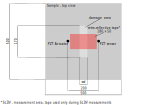
\includegraphics[width=0.95\textwidth]{Chapter_6/sample_dim}
	\end{center}
	\caption{Schematic image of the sample.}
	\label{fig:sample_dim}
\end{figure}

The subject of the parametric study was the effect of the disbond size on the propagating \ac{gw}.
After a reference measurement was made on an intact sample, several measurements were taken for the subsequent damage introduced on the same specimen.
The damage width varied in range \(\mathrm{w_d}=\left [10, 30, 50, 70, 100, 120 \right ]\) \unit{\mm}, while its fixed length was \(\mathrm{l_d} = 175\) \unit{\mm}.
\nomtypeR[w_dam]{\(w_d\)}{Damage width}{}{\unit{\metre}}%
\nomtypeR[l_dam]{\(l_d\)}{Length width}{}{\unit{\metre}}%
The \(N_c=5\) cycle Hann windowed signal at carrier frequencies \(f_c=[50,100,150]\) \unit{\kHz} was used in the measurements.

The data management unit is used to set measurement parameters, managing them, and saving the collected results.
The arbitrary waveform generator (National Instruments, PXI 1095) generates the low-voltage signal from where it feeds Lamb waves detection system (LWDS, Cedrat Technologies) and the actuator (Noliac, NCE51) after 100 times amplification by the  amplifier (Krohn-Hite Corporation, model 7500).
Voltage of the the sensor (Noliac, NCE51) is measured by the oscilloscope (National Instruments, PXI 1095) through the LWDS.
Each measurement was conducted under a temperature of 20\unit{\degreeCelsius} controlled in the environmental chamber (Angelantoni Test Technologies, DM 600C) and averaged 20~times to improve the signal-to-noise ratio.